\section{Software}
To measure an object with a camera, the software has to perform lots of different tasks in a certain period of time.
First off, it needs to take the non linear distortions of the camera into account.
After that, some sort of trigger is needed, to check the frames for objects and pass a frame on, if an object is within the frame.
Now, the software needs to detect a known pattern on the plane where the object lies.
With the known distances of the pattern, a pixel per metric unit can be calculated.
This unit describes, how many pixels in this distance from the camera fit into one metric unit (in this case mm) and is used to convert dimensions in pixel to dimensions in mm and vice versa.
This pattern can also be used to calculate a transformation matrix which compensates for slight angular errors resulting from an imprecise mounting of the camera.
After all these steps, the object has to be recognized.
Finally, the dimensions of the object have to be estimated.

All these steps are described in more detail in the following sections.
For these following sections, it is important to keep in mind, that OpenCV uses a coordinate-system with a switched $x-$ and $y-$axis. 

% listing to python code
\definecolor{codegray}{rgb}{0.5,0.5,0.5}
\definecolor{backcolour}{rgb}{0.95,0.95,0.92}

\lstdefinestyle{mystyle}{
	language=Python,
	backgroundcolor=\color{backcolour},   
	commentstyle=\color{codegreen},
	keywordstyle=\color{blue!50!black},
	numberstyle=\tiny\color{codegray},
	stringstyle=\color{green!50!black},
	basicstyle=\footnotesize\ttfamily,
	breakatwhitespace=false,         
	breaklines=true,                 
	captionpos=b,                    
	keepspaces=true,                 
	numbers=left,                    
	numbersep=2pt,                  
	showspaces=false,                
	showstringspaces=false,
	showtabs=false,                  
	tabsize=2,
	emph={int, char, double, float, range, len, bytes},
	emphstyle=\color{violet},
	morekeywords={as}
}
\lstset{style=mystyle}

\subsection{Initialization}
gobal variables, mapx mapy, init mode

\subsection{Trigger}

\subsection{Edge detection}
morphology

\subsection{Pattern recognition}
The binary image containing the edges is now used to search for the contours of the pattern on the plane.
The pattern consists of 10 rectangles printed on a transparent sheet.
First, it is necessary to find all the contours \texttt{with cv2.findCountours()} inside the two boundaries defined by \texttt{vec} and \texttt{sep}.
This function returns an array of arrays, in which coordinates of the pixels, belonging to one contour are stored.

Because the edge detection is not perfect, some contours will be found which do not belong to the pattern.
By using the area of each contour as basis of decision making, it is possible to remove invalid contours.
This is done in \texttt{remove\_contours()} which is implemented in \texttt{geometry.py}.
If an area of a contour is not between $2600$ and $3400\,$ pixels (both values are passed to the function), the contour is removed.
These two values are of course depended on the rectangle size used and the distance from the camera to the plane.

These left contours (basically an array of points) can be undistorted using \texttt{map\_x} and \texttt{map\_y}.

Now a rectangle is fitted over each contour (with \texttt{cv2.minAreaRect()}).
The center of each rectangle is stored in an array.
These points are here called image-points (in the code as variable \texttt{imgp}).

It is now possible to calculate the pixel per metric unit (\texttt{ppm}) by computing a distance between two image points in pixels and then dividing this distance by the real pattern distance in mm.
In fact it is even more reasonable to do this for a lot of distances and taking the mean of each \texttt{ppm}, assuming that errors in the pattern detection will cancel each other out.

After that, a numpy-array which describes the same pattern how it should appear on the plane if the camera was mounted correctly is generated
This points are here called object-points (\texttt{objp}).
In python this looks like this:
\begin{lstlisting}
	objp = np.array([[-110 * ppm + cx, -75 * ppm + cy],
	                 [ -55 * ppm + cx, -75 * ppm + cy],
	                 [             cx, -75 * ppm + cy],
	                 [  55 * ppm + cx, -75 * ppm + cy],
	                 [ 110 * ppm + cx, -75 * ppm + cy],
	                 [-110 * ppm + cx,  75 * ppm + cy],
	                 [ -55 * ppm + cx,  75 * ppm + cy],
	                 [             cx,  75 * ppm + cy],
	                 [  55 * ppm + cx,  75 * ppm + cy],
	                 [ 110 * ppm + cx,  75 * ppm + cy]], dtype=np.float32)
\end{lstlisting}
where the variables \texttt{cx} and \texttt{cy} are the coordinates of the calibrated principal point of the camera.
The datatype of the entries is forced to float32 because some OpenCV functions do not accept other types.

Now that we have our image- and object points, a perspective transformation matrix can be calculated with
\begin{lstlisting}
	 T, _ = cv2.findHomography(imgp, objp, method=0)
\end{lstlisting}
This function calculates \text{T} in such a way, that the image-points are mapped to the object points using the least-square method (set by \texttt{method=0}).
Or more mathematical:
\begin{align*}
	\begin{pmatrix}
	x_{\text{obj}, i}\\
	y_{\text{obj}, i}\\
	1
	\end{pmatrix}\sim T
	\begin{pmatrix}
	x_{\text{img}, i}\\
	y_{\text{img}, i}\\
	1
	\end{pmatrix}	
\end{align*}
such that
\begin{align*}
	\sum_{i}\left(x_{\text{obj},i}-\frac{T_{11}x_{\text{img},i}+T_{12}y_{\text{img},i}+T_{13}}{T_{31}x_{\text{img},i}+T_{32}y_{\text{img},i}+T_{33}}\right)^2+
	\sum_{i}\left(y_{\text{obj},i}-\frac{T_{21}x_{\text{img},i}+T_{22}y_{\text{img},i}+T_{23}}{T_{31}x_{\text{img},i}+T_{32}y_{\text{img},i}+T_{33}}\right)^2
\end{align*}
is minimized \cite{cv_calib}.
The matrix \texttt{T} is later used to compensate the error made because of the camera mounting. 

\subsection{Object recognition and geometry estimation}
Now that these first calculations are made, the object is detected just like the pattern.
With the function \text{cv2.findcontours()} all contours are extracted from the image with the edges, but this time in between the separation \texttt{sep}.
And again like before, invalid contours are removed, based on their area and undistorted.
because the object in this case is a steel spring, the contours are somewhat complicated and it is possible, that contours are found, which are not connected to each other but definitely belong to the spring.
In this case, the OpenCV function returns them as different contours and it is therefore necessary to combine all returned contours into one single array.
The following code shows how this is achieved in addition with applying the rectification transform and fitting a rectangle over it,
\begin{lstlisting}
	# combine contours to one
	cnts_m = np.concatenate(cnts_m, axis=0).astype(np.float64)
	
	# warp perspective of the contours
	cnts_m = cv2.perspectiveTransform(cnts_m, T)
	
	# minimum area rectangle around cnts_m
	box = cv2.minAreaRect(cnts_m.astype(np.float32))
\end{lstlisting}
where \texttt{cnts\_m} are the contours found previously.
Since now a rectangle with its coordinates is know, everything is ready for the actual geometry estimation.

Because no telecentric objective is used, one has to consider, that the camera looks at the edges of the object in a slight angle.
For simplicity, it is at this point assumed that the steel spring as a cylinder, which is aligned horizontal in the image plane.
A cut through the center of this cylinder along the $y$-axis (OpenCV coordinates) is show in figure \ref{development:diameter}.
\begin{figure}[ht]
	\centering
	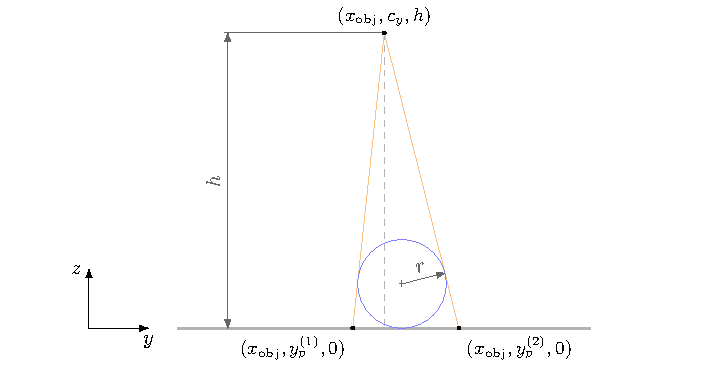
\includegraphics[width=0.9\linewidth]{3-development/software/images/diameter_estimation.pdf}
	\caption{Steel spring cut through the center along $y$-axis\label{development:diameter}}
\end{figure}
$x_{\text{obj}}$ denotes the center of the object (spring) while $cx$ is the $x-$coordinate of the calibrated principal point.
The distance from the camera to the plane can be calculated by using the theorem of intersecting lines, since the focal length and pixel-size are known from the data-sheet of the camera and the pixel per metric unit has been calculated previously.
Also known are the two observed points on the plane $(x_{\text{obj}}, y_p^{(1)})$ and $(x_{\text{obj}}, y_p^{(2)})$.

The distances from these two points on the plane to the camera and to each other can now be calculated as
\begin{align*}
	d_{1}&=\sqrt{(c_y-y_p^{(1)})^2+h^2}\\
	d_{2}&=\sqrt{(c_y-y_p^{(2)})^2+h^2}\\
	d_{3}&=y_p^{(2)}-y_p^{(1)}.
\end{align*}
The distance must of course have the same units, in this case all distances in pixel where first converted to distances in mm.

This provides enough information to apply the geometry of in-circles \cite{incircles} to calculate the radius of the object as
\begin{align*}
	r=\sqrt{\frac{(s-d_1)(s-d_2)(s-d_3)}{s}}
\end{align*}
with
\begin{align*}
	s=\frac{d_1+d_2+d_3}{2}.
\end{align*}

A similar principle is applied to calculate the length of the object.
Figure \ref{development:length} where again
$y_{\text{obj}}$ denotes the center of the object (spring) while $c_x$ is the $x-$coordinate of the calibrated principal point.
\begin{figure}[ht]
	\centering
	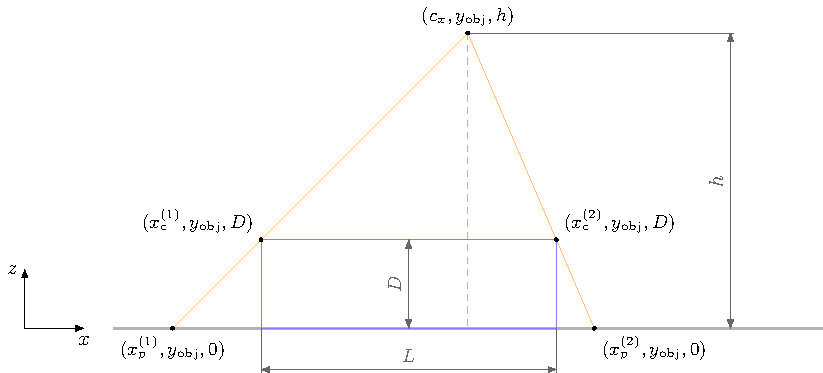
\includegraphics[width=0.9\linewidth]{3-development/software/images/length_estimation.pdf}
	\caption{Steel spring cut through the center along $x$-axis\label{development:length}}
\end{figure}
Observed are the two points on the plane $(x_p^{(1)}, y_{\text{obj}})$ and $(x_p^{(2)}, y_{\text{obj}})$.
But simply taking the difference of $x_p^{(1)}$ and $x_p^{(2)}$ result in to long length estimation.

Since $h$ is know, and $D$ has been calculated previously ($D=2r$), the theorem of intersecting lines allows one now to make the correction from the coordinates on the plane ($x_p^{(k)}$) to the points on the edge ($x_c^{(k)}$).

Mathematically expressed this results in
\begin{align*}
	\frac{c_x-x_c^{(k)}}{c_x-x_p^{(k)}}=\frac{h-D}{h}\quad\Leftrightarrow\quad
	x_c^{(k)}=\frac{h-D}{h}(c_x-x_p^{(k)}).
\end{align*}
After this correction the length can be calculated as
\begin{align*}
	L=x_c^{(2)}-x_c^{(1)}.
\end{align*}

These calculations are only accurate, if the object is placed horizontal in the frame.
In order to make accurate estimations even if the object is slightly rotated, the angle ($\theta$) between the minimum area rectangle found around the object and the horizontal has to be calculated.

The object or respectively the rectangle (the four corner points) has to be moved to the coordinate origin by removing the center and then rotated.
This transformation can be expressed as
\begin{align*}
	\begin{pmatrix}
	x'\\
	y'\\
	\end{pmatrix}=
	\begin{pmatrix}
	\cos(\theta)&-\sin(\theta)\\
	\sin(\theta)&\cos(\theta)
	\end{pmatrix}
	\begin{pmatrix}
	x-x_{\text{obj}}\\
	y-y_{\text{obj}}\\
	\end{pmatrix},	
\end{align*}
where $(x, y)^T$ are coordinates of the points of the object, $(x', y')^T$ are transformed coordinates and $(x_{\text{obj}}, y_{\text{obj}})$ are again the coordinates of the center of the object, or respectively the min area rectangle.
By applying this transformation beforehand, the geometry estimation is independent of the the angle the object has to the horizontal. 

\subsection{Compensation of the rolling shutter}


